\subsection*{Hra po Praze 2019 z pohledu organizátorů}
\label{sub:hra_po_praze_2019_z_pohledu_organizátorů}

Letošní Hra po Praze byla ta nejsofistikovanější, nejpřipravovanější a z realizační stránky i nejtěžší hra z těch tří, co jsem zatím dělala. První porada proběhla 14.10. a od té doby jsme měli další čtyři porady a jednu přespávačku. Celkově se na vymýšlení a organizaci podílelo devět uďů a mnoho dalších bylo na místě. Celý měsíc a půl jsme intenzivně vymýšleli zápletku, sháněli materiály, verbovali externisty… zkrátka přípravám jsme věnovali mnoho času.

Co se týče samotné realizace HpP, možná jsme si dali příliš málo času pro realizaci na místě (proto někteří patroni přišli pozdě na sraz skupinek), takže byl začátek poměrně zmatený a hektický. Já osobně jsem se nervovala úplně maximálně, hih. Celou dobu jsme byli v lehkém časovém skluzu, ale nakonec jsme jej dohnali, takže zakončující bitva vyšla přesně, za což jsem byla já osobně velmi ráda. 

\clearpage

Ale i tak - přes veškerý stres a strach z neúspěchu nebo úplného sesypání hry - se Hra dle mého názoru vydařila a věřím, že si ji děti i spousta uďů užilo. Což považuju za nejlepší výsledek, jaký mohl nastat.


\begin{center}

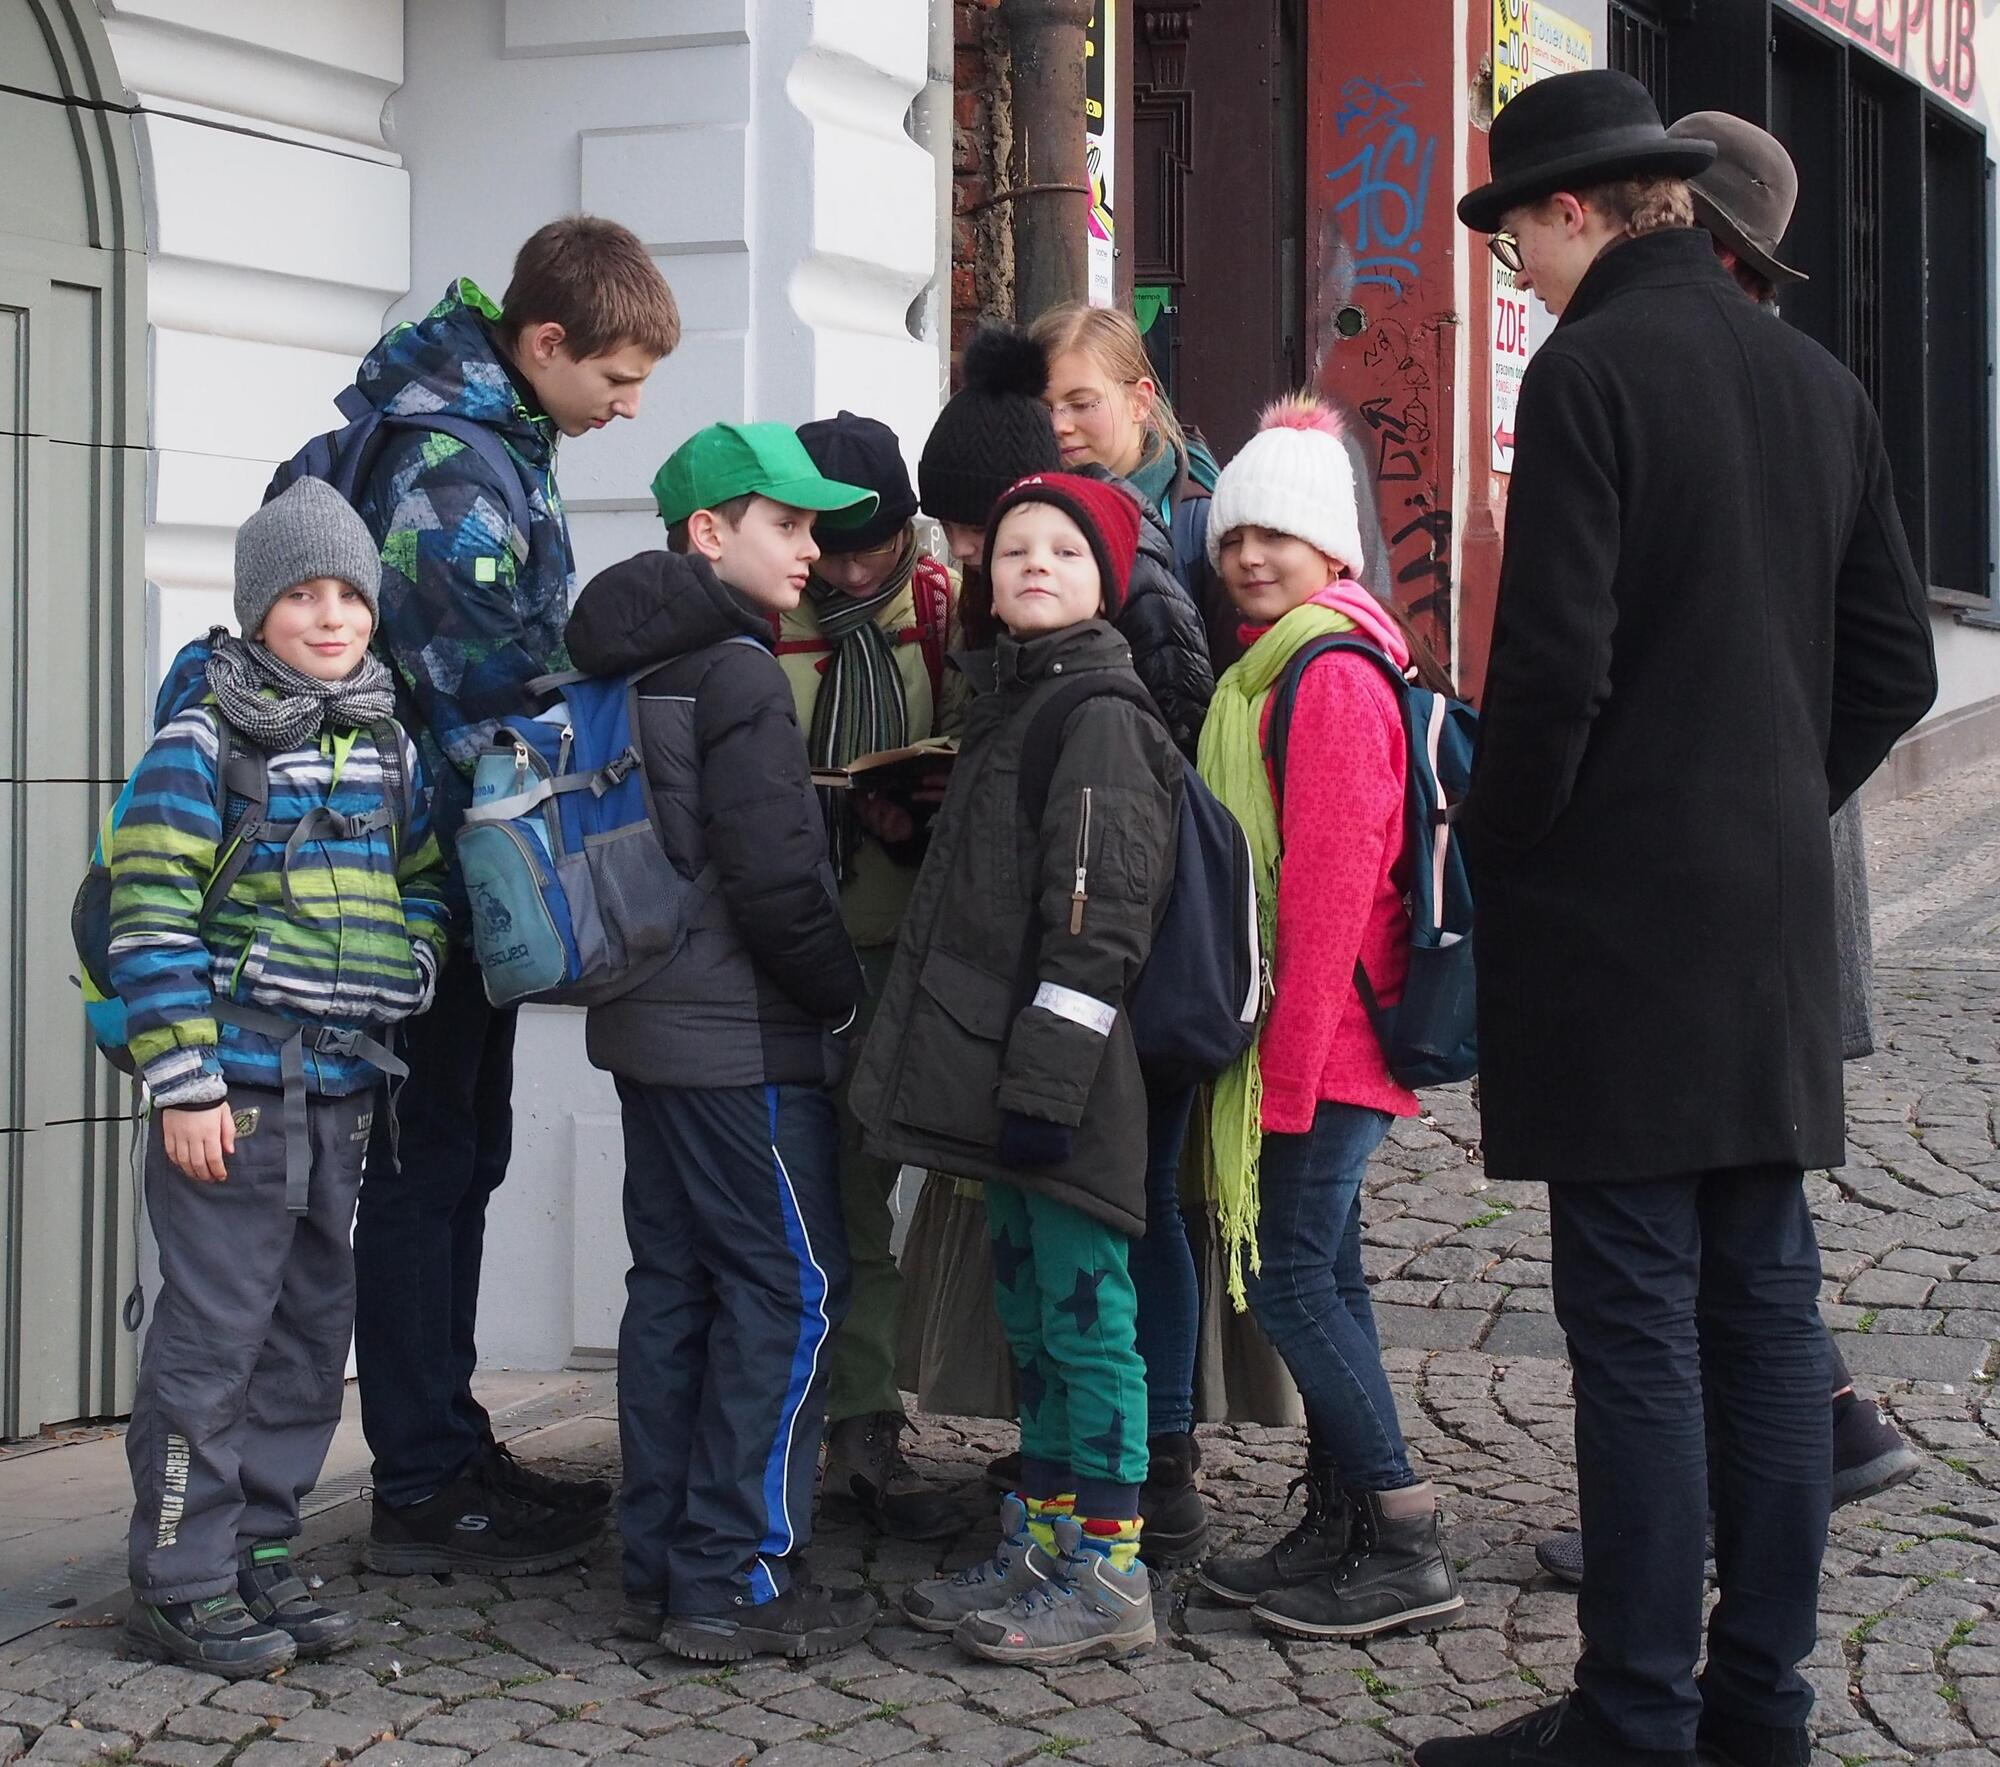
\includegraphics[width=8cm]{img/udo_clanky/hrapopraze.JPG}

\end{center}
\podpis{Štípadlo}
\clearpage